%*********************第二章******************
\chapter{心脏组织模拟在大规模异构多核节点平台下的并行优化}
\label{chapbmvc}

\section{引言}
绪论已经介绍过,视觉跟踪器是视频监控、人机交互、智能导航等应用领域至关重要的基础。
从上世纪80年代的KLT跟踪器\upcite{lkoptflow, klt2},到最新提出的深度学习跟踪器\upcite{deepimage, deeptrack},
视觉跟踪已经被研究了几十年。
但随着应用需求的不断提升,应用场景的日趋复杂,很多问题仍然未得到有效解决。
跟踪器对目标物体的尺度和宽高比的适应力就是这些问题之一。

过多的非目标物体信息可能包含在边界框中,而部分目标物体信息却可能在边界框外。
这些误差将在物体描述中积累,积累到一定程度,跟踪器将出现偏移(Drifting),整个跟踪过程很可能就此失败。
图\ref{scalearerror}就展示了一个尺度和宽高比误差的可视化例子。
因此,跟踪器对目标尺度和宽高比的适应力对跟踪精度有着决定性的作用。

\begin{figure}[htb]
\centering
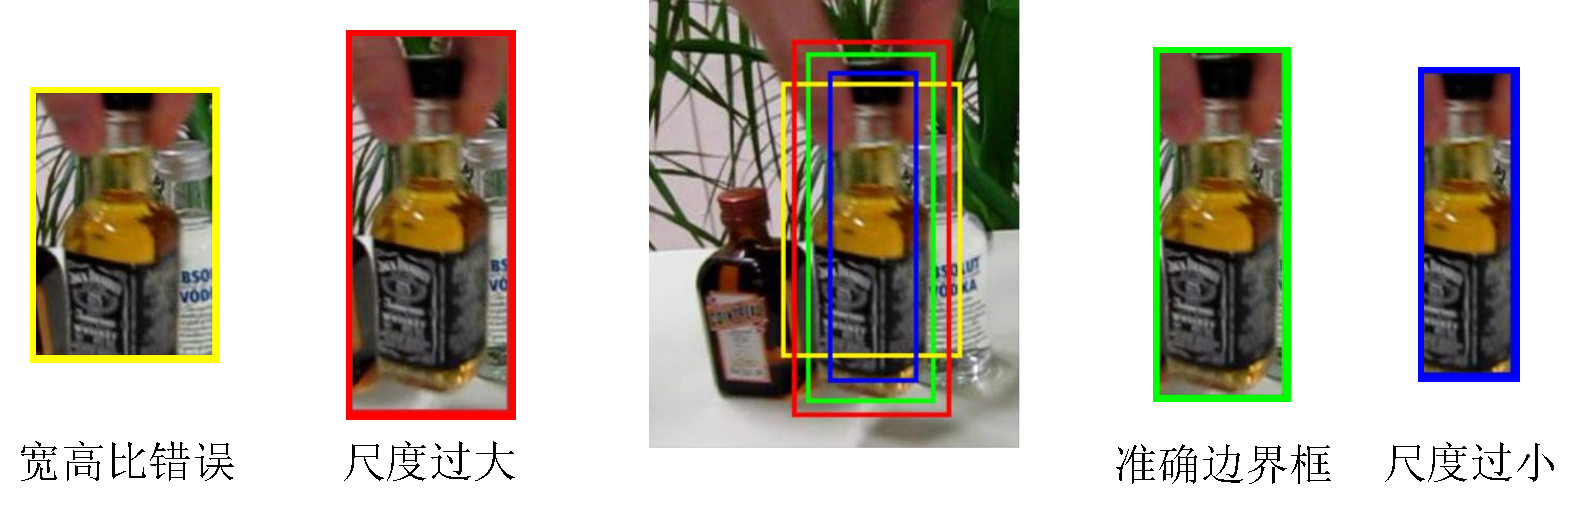
\includegraphics[width=12.5cm]{scaleaspect.pdf}
\caption{尺度和宽高比误差的可视化例子}
\label{scalearerror}
\end{figure}

为了应对视觉跟踪应用中的诸多挑战,跟踪算法正变得越来越复杂。
然而近年提出的基于相关滤波的跟踪器\upcite{cfsurvey, mosse,csk,kcf,dsst,act,samf,pbcf} 在取得上佳性能的同时,却十分简单和快速。

但是,滤波器的输入必须是固定大小的图像块,因此基于相关滤波的跟踪器天生缺乏对于目标尺度和宽高比变化的适应力。
尽管一些能够适应尺度变化的变型\upcite{dsst,samf,pbcf}已经出现,但是它们仍局限于预定的尺度采样方式,不够灵活。
此外,在本章已知的范围内,除了\cite{pbcf}以外还没有相关滤波跟踪器能够解决对于目标宽高比的适应性问题。

在物体检测领域,近来具有顶级性能的物体检测系统\upcite{rcnn,spp}均采用了``目标候选''方法来提取可能包含目标物体的候选区域。
该类方法可以在没有任何先验知识的情况下,在输入图像中提取任意尺度、宽高比的候选边界框,如图\ref{detectionproposalres}所示。
目标候选方法不仅能够避免对大量的边界框进行分类,还能预先滤除大部分错误的边界框,大幅提高检测精度\upcite{dpsurvey,dpcompare}。
在本章中,目标候选生成器EdgeBoxes\upcite{edgeboxes}将被融入跟踪器中,
以提升跟踪器对尺度和宽高比的适应力。

\begin{figure}[htb]
\centering
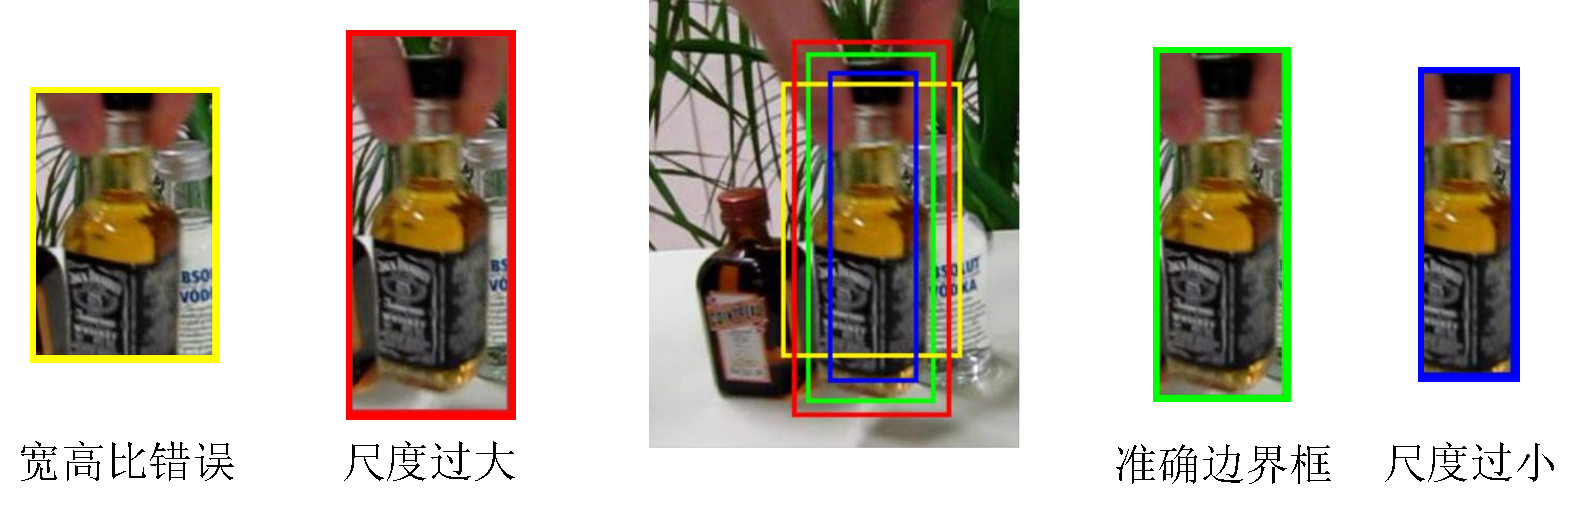
\includegraphics[width=13cm]{scaleaspect.pdf}
\caption{生成``目标候选''的可视化例子}
\label{detectionproposalres}
\end{figure}

本章的内容安排如下:第2节介绍与本章紧密相关的现有研究工作;
第3节介绍本章跟踪器框架的基础\pozhehao 核化相关滤波器KCF;


\section{相关研究}
\subsection{心脏组织模拟的数学模型}
根据绪论中对跟踪器各模块的功能分析可以看出,运动模型是决定一个跟踪器的尺度和宽高比适应力的关键。
\cite{survey51}中的跟踪器基于光流跟踪算法,已被广泛应用于图像对准(Image Registration)。
它通过增量式对齐(Incremental Alignment)来计算两帧中目标物体图像块的仿射变换(Affine Transformation)。
由于仿射变换的参数包含6个自由度,因此该跟踪器可以感知目标物体的位移、尺度变化和旋转。
LSK跟踪器\upcite{lsk}在每一帧中都会预先``猜测''一个目标中心位置并采样候选图像块,


\subsection{心脏组织模拟的并行实现}
因此,密集采样的模式(例如采样时边界框的大小、形状是否可变)决定了跟踪器对尺度和宽高比的适应力。
MOSSE跟踪器\upcite{mosse}将经过随机仿射变换的目标物体图像作为训练集,用于初始化它的相关滤波器。
但是在跟踪过程中,采样边界框的尺度和宽高比不再变化,滤波器仅用于检测目标的当前位置。
KCF\upcite{kcf}跟踪器是CSK\upcite{csk}的一个扩展版本,它通过利用图像块中的循环模式进行卷积操作,取得了极高的跟踪效率。
KCF还利用``核技巧(Kernel Trick)''来增强了传统的相关滤波器,同时使得滤波器支持多通道的特征。
但是,它仍然没有解决尺度的适应力问题。

\section{心脏组织模拟的数学建模}


\section{心脏组织模拟的高性能并行实现}

 \subsection{心脏组织模拟的tissue-级并行}
 
 \subsection{心脏组织模拟的cell-级并行}

\subsection{心脏组织模拟的dyad-级并行}

\subsection{心脏组织模拟中随机数生成}



\section{实验结果与分析}
\subsection{实验设置}


\subsubsection{心脏组织模拟单设备性能}
\label{datasetcomponetsec}
本章的测试集来自著名的OTB,它包括了50个极具挑战性的视频序列(共计51个跟踪目标),其概览如图\ref{otb50}所示。
OTB还为每一个视频序列注明了其主要包含的跟踪障碍,例如``快速运动''、``遮挡''、``尺度变化''、``光照变化''等共计11种,
且一个视频序列可能包含多种跟踪障碍。



\subsection{心脏组织模拟的单节点性能}

\subsection{心脏组织模拟的多节点性能}

\section{小结}
该方法将用于把更多的目标候选生成器和跟踪器相结合,以深入研究目标候选在视觉物体跟踪中的作用和潜力。
此外,本章并未对目标候选生成算法进行优化,下一章将针对跟踪任务的需求,对目标候选生成器进行深入改进。
